\chapter{Définition des structures}


\section{Les structures}
La résolution du problème requiert des structures de données afin de représenter :
\begin{itemize}
\item des coordonnées, représentées par la structure \verb$Coordonnees$ (voir \ref{Coordonnees_8h}) contenant deux entiers $x$, l'abscisse, et $y$, l'ordonnée et permettant de situer une case dans un puzzle ;
\item des indices, représentés par la structure \verb$Indice$ (voir \ref{operationLInd_8h}) contenant la valeur d'une case et sa coordonnée ;
\item un ensemble d'indices représenté par une liste ;
\item un ensemble de coordonnées également représenté par une liste ;
\item l'ensemble des «~cases~» contenant les indices et la liste des voisins possibles pour cet indice ;
\item la grille correspondant à l'image résultat (donnant donc les cases «~noircies~»).
\end{itemize}
Nous avons choisi de représenter ces deux derniers points par une unique structure \verb$TabVoisins$.

\subsection{Les listes chainées}
Nous avons défini deux types de listes chainées : les listes de coordonnées et les listes d'indices.

De façon générale, la liste est composée d'une donnée, sa première valeur, et de l'adresse de l'élément suivant :
\begin{itemize}
\item \verb$ListeCoord$ (voir \ref{operationLCoord_8h}) est donc une liste dont les éléments sont des \verb$Coordonnees$ ;
\item \verb$ListeInd$ (voir \ref{operationLInd_8h}) est, elle, une liste d'\verb$Indice$.
\end{itemize}

Les principales fonctions associées aux listes sont celles de création (constructeur / destructeur), d'insertion et de suppression.
Tout d’abord, la fonction \verb|creerLCoord|, respectivement \verb|creerLInd|, permet la création d’une liste. Elle prend donc en paramètre l'élément tête de la liste ainsi qu'une liste équivalente à la queue de la liste que l'on souhaite créer et pouvant être égale à la liste vide. 
La fonction \verb|detruitLCoord| (respectivement \verb|detruitLInd|) supprime l’intégralité de la liste passée en paramètre.
Les fonctions d’insertion permettent, elles, d’ajouter un élément dans la liste, soit au début soit à la fin.
Enfin, les fonctions de suppression (comme \verb|supprimerpremierLCoord| ou \verb|supprimerdansLCoord|) permettent d’enlever soit le premier soit un élément quelconque de la liste.
Ces deux derniers types de fonctions ne renvoient rien mais modifient des listes.

Ces listes sont définis dans les modules d'opération sur les listes de coordonnées et d'indices situés respectivement dans les fichiers \verb$operationLCoord.h$, \verb$operationLCoord.c$, \verb$operationLInd.h$ et \verb$operationLInd.c$ (voir \ref{graphes-dependance}).

\subsection{Un tableau de voisins}

La structure \verb$TabVoisins$, définie dans les fichiers \verb$TabVoisins.h$ (\ref{TabVoisins_8h}) et \verb$TabVoisins.c$ (voir \ref{graphes-dependance}), est un tableau de cases qui donne pour chaque case sa valeur et la liste de ses potentiels voisins. Pour cela, elle utilise la structure \verb$CaseVoisins$ (voir \ref{TabVoisins_8h}) associant donc :
\begin{itemize}
\item la valeur d'une case, qui peut être : 
	\begin{itemize}
	\item 0 si la case est libre ;
	\item 1 si la case est un indice de valeur 1 ou une case empruntée par un chemin ; 
	\item $n > 1$ si la case est un indice de valeur $n$.
	\end{itemize}
\item sa liste \verb$ListeCoord$ qui est la liste des coordonnées des voisins de la case si celle-ci est un indice de valeur supérieure à 1. 
\end{itemize}
\verb$TabVoisins$ a également en donnée les dimensions du puzzle d’origine.

\begin{figure}[h]
 \centering
 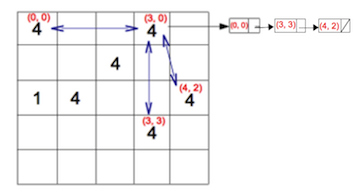
\includegraphics{structures1b}
\caption{Exemple de TabVoisins avec la case $(3, 0)$ qui a la valeur 4 et sa liste de voisins possibles}
\end{figure}

On utilise sur cette structure des fonctions «~basiques~» de création et d'accesseurs :
\begin{itemize}
\item \verb|new_TabVoisins_from_Probleme| qui permet de créer un nouveau TabVoisins représentateur d’un problème donné ;
\item \verb|TabVoisins_getWidth| qui renvoie sa largeur ;
\item \verb|TabVoisins_getHeigth| qui renvoie sa hauteur ; 
\item \verb|TabVoisins_setValeurs| qui permet d'assigner une valeur à une case existante ; 
\item \verb|TabVoisins_getValeurs| qui renvoie la valeur d'une case existante ;
\item \verb|TabVoisins_setVoisins| qui permet de spécifier les voisins potentiels d'une case ; 
\item \verb|TabVoisins_getVoisins| qui renvoie la liste des voisins possibles d'une case.
\end{itemize}
